% Earth inside the models: ExoPlaSim 3.4.2, CM1 r22 with WRF-ELEC, SWAN 41.51 and SWASH 12.01 adapted to a breathable Moon
% Paper ID e8b42cb5-48da (UUIDv4 e8b42cb5-48da-402c-b261-4de808e9062a). Built with `make` in this folder.
\documentclass[11pt]{article}
\usepackage[a4paper,margin=25mm]{geometry}
\usepackage[T1]{fontenc}
\usepackage{newtxtext,newtxmath}
\usepackage[utf8]{inputenc}
\usepackage{microtype}
\usepackage{graphicx}
\usepackage{booktabs,tabularx,array,makecell}
\usepackage{siunitx}
\usepackage{xcolor}
\usepackage[font=small,labelfont=bf,labelsep=period]{caption}
\usepackage{enumitem}
\usepackage{csquotes}
\usepackage[style=authoryear,maxcitenames=2,maxbibnames=10,minbibnames=7,uniquelist=false,giveninits=true,
            doi=true,url=false,isbn=false,backend=biber]{biblatex}
\usepackage[hidelinks,breaklinks]{hyperref}
\usepackage{orcidlink}
\addbibresource{references.bib}
\setcounter{secnumdepth}{0}          % unnumbered headings throughout
\sisetup{group-minimum-digits=4,range-phrase=--,per-mode=symbol}
\setlist{nosep,leftmargin=*}
\renewcommand{\arraystretch}{1.15}
\newcolumntype{L}{>{\raggedright\arraybackslash}X}
% A claim marker: renders nothing, lets the checker trace each number to paper/claims.json.
\newcommand{\claim}[1]{}
\newcommand{\code}[1]{\texttt{\small #1}}

\title{\textbf{Earth inside the models: ExoPlaSim 3.4.2, CM1 r22 with WRF-ELEC, SWAN 41.51 and SWASH 12.01 adapted to a breathable Moon}}
\author{Daniel S. Goldman\,\orcidlink{0000-0003-2835-3521}}
\date{Draft, \today. Paper ID e8b42cb5-48da}

\begin{document}
\maketitle
\begin{abstract}
\noindent Exoplanets and constructed worlds whose air and water resemble Earth's, while their gravity, size,
day or starlight differ, are studied with models built for Earth, in which an Earth value left in the code runs
without failing. Four such models were adapted to a breathable Moon, which changes gravity, column mass, scale
height and day length together: ExoPlaSim~3.4.2, CM1 release~22 with WRF-ELEC's electrification, SWAN~41.51
and SWASH~12.01. The adaptation found Earth values in four forms (constants, units of time, geometry, and fits
beyond their range) and five defects in the released codes. Three defects produce little or no error at
Earth's values and affect other users' runs: ExoPlaSim's Sun clock, which skipped back 32.5\textdegree\ each
lunar model day;\claim{H23} its convective-cover unit, which also biases synchronous runs;\claim{W06} and its
default orbit, which replaced the Moon's tilt with Earth's. General repairs correct units, apply scaling
laws or remove defects and serve other worlds unchanged; a method computes the curved geometry for each world's
column; and calibrations to an in-house line-by-line model hold near the design case. Identity, reproduction, similarity and benchmark checks test the code; the lunar climate is
unobserved. On the case, the general repairs moved the global mean by a few kelvin and the distribution of rain
further, the calibrations and PlaSim's Earth-tuned cloud and longwave cooling moved it most,\claim{G05} and the
storms' freezing level stood five to six times higher than Earth's, their lightning rarer and
larger.\claim{G09}\claim{G10} Building those parts from the reference's physics and from cloud-resolving runs
would narrow the Moon's uncertainty and widen the models' reach together.
\end{abstract}

\section{Introduction}

Some exoplanet climate studies hold a planet's air close to Earth's and change the planet around it.
\textcite{yang2014strong} and \textcite{way2018climates} slowed the rotation of planets with Earth-like air
and followed their cloud and temperature as the day lengthened, \textcite{thomson2019effects} varied the
gravity of a terrestrial planet in moist and dry general circulation models, and
\textcite{boutle2017exploring} placed an Earth-like atmosphere on Proxima Centauri~b, under a cooler star.
Work on constructed worlds asks how a planet could be made habitable \autocite{mckay1991making} and, for a
designed world, what its climate would be \autocite{goldman2026terluna}. Many of the models used in such
work descend from Earth models: ROCKE-3D from the GISS ModelE2, ExoCAM from NCAR's Community Atmosphere Model
and ExoPlaSim from the Planet Simulator \autocite{way2017resolving,wolf2022exocam,paradise2022exoplasim}; the
cloud-resolving models SAM and CM1 have simulated convection on tidally locked planets and in pure-steam air
\autocite{yang2023cloud,tan2021convection}; and SWAN, a coastal wave model, has been run for the ancient
seas of Mars \autocite{banfield2015winds}.

The developers of several such ports found values fixed for Earth in the code. PlanetWRF's developers,
finding WRF written to apply to Earth alone, redefined its second as 1/86,400 of the planet's rotation;
TitanWRF's removed hard-wired Earth settings from the physics; and ROCKE-3D's found constants tied to the
lengths of Earth's day and year, then eliminated or generalised its Earth-centric options one by one in a
second release, measuring the effect of each
\autocite{richardson2007planetwrf,newman2011stratospheric,way2017resolving,tsigaridis2025rocke3d}.
ExoPlaSim's description records that the Planet Simulator's solar day had to be taken out of its unit
conversions before slow rotators could be run, and that its near-infrared water absorptivity is tuned to a
solar spectrum \autocite{paradise2022exoplasim}. In each of these ports the developers repaired what their own
world required, and the developers of THOR, a model written for other planets from the start, describe planet-specific
tunings as often built into codes and hard to find \autocite{deitrick2020thor}. On an Earth-like
world, an Earth value left in the code can go unnoticed: the air and water stay within the regime the model
was built for, so a constant set for Earth's gravity, or a formula that counts rain per Earth day, runs to
completion and returns a plausible number. A modeller studying such worlds needs to know where a model's
Earth values lie and which repairs made for one world hold on another.

The work reported here took up both questions on one world, a breathable Moon designed in an open project
\autocite{goldman2026terluna}, with 1.2~atm of nitrogen and oxygen at the water level, seas over 28\% of the
surface, sunlight filtered by a shield in space, and the Moon's own gravity of \SI{1.62}{m.s^{-2}} and
29.53-day solar day.\claim{S01} Its air is close to Earth's, while four ratios on which the models' Earth
values depend lie far from Earth's at once: the air over each square metre is 7.25 times
Earth's,\claim{S02} the scale height of about 52~km is 23 times Earth's in proportion to the
radius,\claim{S03} gravity is a sixth of Earth's, and the solar day lasts 29.5 Earth days. Adapting models
to this world exercised many of the Earth values they hold, with errors large enough to measure: the horizon
air mass that PlaSim fixes at Earth's 35, for one, is about 7 for the Moon's well-mixed air.

The global climate comes from ExoPlaSim~3.4.2 \autocite{paradise2022exoplasim,paradise2025exoplasim}, the
Planet Simulator \autocite{fraedrich2005planet} extended for other worlds, which runs decades of lunar
climate in an hour or two on four processor cores\claim{S14} and diagnoses its clouds and convection from
formulas fitted to Earth. Slices of that climate force CM1 release~22 \autocite{bryan2002benchmark,bryan2026cm1}
on rings of columns along latitude circles or tilted great circles and in doubly periodic boxes, where it
resolves the convection the GCM diagnoses and forms its own clouds and rain; with the electrification of WRF-ELEC grafted in
\autocite{mansell2010simulated,fierro2013implementation,mansell2026wrfelec}, it also separates charge and
makes lightning. The GCM's surface stress drives SWAN~41.51 \autocite{booij1999third,swan4151user} over the
seas, and SWAN's spectra drive SWASH~12.01 \autocite{zijlema2011swash,swash1201user} up the shore. The
radiation of both atmospheric models was tested against an in-house line-by-line radiative--convective model
built on HITRAN lines as served in September 2026 \autocite{gordon2022hitran2020} and the MT\_CKD continuum
\autocite{mlawer2012development}: the GCM's was calibrated to it, and CM1's checked against it. Each
model's grid, levels, time step and runs are given in Table~\ref{tab:config}.

Adapting the four models found Earth values in four forms, dimensional constants written into the code,
units of time, geometry, and empirical fits and simplifications used beyond the range they were made for, and
five defects in the released codes, three of which produce little or no error at Earth's values. Each repair
falls into one of three classes with different reach: a general repair, which corrects a unit, applies a
scaling law or a physical law, or removes a defect, and which another world takes unchanged; a general method with
a table computed for each world's column, as for the curved geometry of a tall air; and a calibration, whose
coefficients were fitted to the reference model on the columns of the lunar design case and are fitted again
for any other world. On the case, the repaired models measure how far each Earth value moved the climate and
which of those that remain move it most, and the three classes set which other worlds the adapted models can
reach. Every lunar climate number is a conditional model result, holding given the scenario and the Earth
values that remain; with the lunar climate unobserved, the strongest test open to these numbers is agreement
among independent models.

\section{A breathable Moon as a modelling regime}

The models take Terluna's design scenario as fixed conditions. The air holds 121,590~Pa at the water level,
with oxygen at Earth's partial pressure of 21,227~Pa (17.5\% of the air), argon in Earth's ratio to nitrogen,
400~ppm of carbon dioxide and nitrogen for the balance; the land stands above the water level, so the
global-mean surface pressure is 1.16~atm and ranges from 1.02 to 1.22~atm.\claim{S05} Seas fill the lunar
basins to 28\% of the surface and rain-fed lakes stand at their own levels, so 759 of the GCM's 2,048
cells, 40\% of its surface, hold water.\claim{S06} Sunlight is the TSIS-1 solar spectrum
\autocite{coddington2021tsis} passed through a titania shield in space, 1,235~W\,m$^{-2}$ at the top of the
air, dimmed evenly at every wavelength to 1,198~W\,m$^{-2}$ in the design case; the shield removes the
ultraviolet that would make ozone, so the air carries none.\claim{S07} The land has a placeholder albedo of
0.2 and the seas a 50~m slab with sea ice. Every climate number below holds given these choices; they are a
design, and other designs would move the numbers.

\begin{table}[t]
\caption{The ratios that separate the Open Moon from Earth, and the model parts each strains. Lunar values
are for the 1.2~atm design case; scale heights use the surface temperature and the air's mean molar mass;
horizon air masses are Chapman's grazing factor $\sqrt{\pi R/2H}$ for an isothermal air, which PlaSim's code
sets at 35 for Earth. The convective grid is a nominal scale from the dry dynamics' similarity.}
\label{tab:regime}
\small
\begin{tabularx}{\textwidth}{@{}lrrL@{}}
\toprule
Quantity & Earth & Open Moon & What it strains \\
\midrule
Surface gravity (m\,s$^{-2}$) & 9.81 & 1.62 & Dynamics; fall speeds; sea roughness; wave dispersion; heights in pressure terms \\
Surface pressure at the water level (bar) & 1.01 & 1.22 & RRTMG's tables, whose highest pressure is 1.05~bar \\
Air over each square metre (t) & 10.3 & 74.9 & Broadband absorber paths fitted on Earth's \\
Scale height at the surface (km) & 8.4 & 52 & Every height-based formula \\
Scale height over radius & 0.0013 & 0.030 & Flat, sunlit-only columns; the thin shell \\
Horizon air mass of well-mixed air & 34.5 & 7.2 & Earth's slant factor, fixed in PlaSim \\
Solar day (Earth days) & 1 & 29.53 & Formulas written per day; the soil's thermal wave; the model calendar \\
Sidereal rotation (Earth days) & 0.997 & 27.32 & ExoPlaSim's Sun clock; the Coriolis parameter \\
Tilt of the equator (\textdegree) & 23.44 & 1.54 & ExoPlaSim's orbit default \\
Height of the 0\,\textdegree C level (km) & 4.5--5 & 25 & Ground-strike rules; the charging zone \\
Tops of deep storm cloud (km) & 15--18 & 55--80 & Model tops; the levels of cold cloud \\
Fall speed of rain, relative & 1 & 0.34 & Evaporation of falling rain \\
Grid for deep convection (km) & 1 & 6 & Cost; the meaning of a resolution \\
\bottomrule
\end{tabularx}
\end{table}

Table~\ref{tab:regime} sets out what the scenario does to the ratios the models depend on. The air over
each square metre, 7.25 times Earth's, stretches every absorber path: water vapour reaches
170~kg\,m$^{-2}$ in the design case and 348~kg\,m$^{-2}$ in its warmest test, where Earth's column holds
about 25 \autocite{trenberth2005trends}.\claim{S08} The scale height, about 52~km against a radius of
1,737~km, makes a poor picture of the Moon's air out of the geometry the radiation codes assume, a stack of
flat layers lit only while the Sun stands above each column's horizon. The air's mass sits on average
48.6~km up, a shell 50~km up has 5.8\% more area than the ground beneath it, and straight rays through the
design column give a horizon air mass of 7.1 for well-mixed air and 13.5 for water vapour, where PlaSim's
formula, written for Earth, gives 35.\claim{S09} The same height that curves the radiation's paths also
strains the dynamics' thin shell: gravity at the 86~km tropopause is 9\% below its surface value, a column
with gravity falling as $GM/r^2$ holds about 5\% more air per unit area than $p_s/g_s$, and the widening
shells hold 11.5\% more over each square metre of ground.\claim{S10}

Gravity and the calendar strain everything else. A sixth of Earth's gravity raises every pressure level
sixfold in height, so a formula written in metres puts its features six times too low; it slows the fall
of droplets sixfold, of rain about threefold and of graupel 2.3-fold; it sets the roughness length of a
wind-driven sea six times longer for the same friction velocity \autocite{charnock1955wind} and slows a
deep-water wave of a given length to 0.41 of its speed on Earth.\claim{S11} The dry dynamics stretch about
sixfold in size and duration at the same speeds, so a 6~km column of a cloud-resolving model stands for
about 1~km at Earth's scale; the microphysics and the radiation keep their own scales, and the gravity pair
meant to test the stretch failed to convect.\claim{S12} The 29.53-day solar day deepens the soil's thermal
wave to about 0.6~m, $\sqrt{29.53}\approx5.4$ times the depth of Earth's diurnal wave, and multiplies nearly
thirtyfold whatever a formula counts per day; the 27.32-day rotation, slow against the Sun but synchronous
with Earth, sets a Coriolis parameter of $\SI{5.2e-6}{s^{-1}}$ at 80\textdegree, an inertial period of
14 Earth days.\claim{S13} The tilt of 1.54\textdegree\ leaves the poles a grazing Sun all year, a regime
that ExoPlaSim's orbit default would replace with Earth's seasons.

The questions each model owns follow from these strains. How warm and humid the air near the ground, where
people and plants would live, runs through the month-long day, how much rain falls and where, and what the
Moon's mean climate becomes under each change of shield or gas: the GCM answers these for the whole Moon,
with clouds diagnosed from Earth formulas. How storms build, how much of their rain reaches the ground and
how the lowest kilometres differ from the GCM's: CM1 answers these where it forms its own clouds. How often
lightning strikes and what each flash carries: the electrified CM1. How high the seas run and what reaches
each shore: SWAN and SWASH, driven by the GCM's stress. The line-by-line model stands behind the
atmospheric models, holding the radiation the GCM is calibrated to and CM1's is checked against.

\section{Where Earth hides in the models}

A model carries Earth wherever one of its values or forms agrees with Earth because Earth set it, and
such a part, run on the Moon, returns Earth's answer to a lunar question. Table~\ref{tab:inventory} lists
the instances found on the paths the lunar runs use, each with its form and its state at Terluna commit
186b294; the defect log in the accompanying repository adds those found off those paths and gives each
one's discovery, evidence, repair and measured effect. The inventory separates two kinds. In a limitation
the code does what it was written to do, on the world it was written for. In a defect the code is wrong on
its own terms, on every world. Four of the five forms are limitations; the fifth holds the released codes'
defects.

\textbf{Constants written into the code.} A dimensional constant carries the scale of the world it was
set on, and gravity is the commonest. CM1 release 22 sets it to 9.81~m\,s$^{-2}$ in four places on the
lunar cases' paths, its dynamics, the conversion of pressure to layer mass in its RRTMG radiation
\autocite{iacono2008radiative}, its CAPE diagnostic and the Morrison microphysics, and in several schemes
those cases leave unselected; Morrison's fall-speed laws $V = aD^b$ and their caps hold Earth's gravity in
their coefficients.\claim{H01} WRF-ELEC's NSSL scheme sets 9.8 twice and ties the ventilation of
evaporating rain and depositing ice to Earth's fall-speed coefficients.\claim{H02} Earth sets two thresholds
and a time step in WRF-ELEC's lightning. A breakdown field scaled with the air's density
\autocite{dwyer2003fundamental} and capped at 180~kV\,m$^{-1}$ acts on Earth only below about 4.5~km,
beneath where flashes start, and in lunar air below about 36~km, where it lowers the field by 44\% at the
ground. A ground strike is declared when a channel reaches air warmer than $-7$\,\textdegree C, about 5~km
above Earth's ground and 27--34~km above the Moon's. A 0.75~s sub-step is sized for 500~m layers and
Earth's fall speeds.\claim{H03} Earth's seas set SWAN's constants. It reduces its linear wind input above a
knee fixed at 1~Hz, a value its source comments call largely arbitrary, and the fixed knee breaks the
model's gravity similarity: stock SWAN misses a sixfold similarity test by
5.44\% in significant wave height.\claim{H04} It also fixes the air's density at 1.28~kg\,m$^{-3}$, where the air over the lunar seas
holds about 1.40.\claim{H05} Earth's composition and rotation complete the set: RRTMG takes carbon dioxide
from the calendar year and carries Earth's methane, nitrous oxide, halocarbons and ozone, and CM1's beta
plane derives its gradient from Earth's rotation and a 6,370~km radius.\claim{H06} Each constant is right
for Earth, and can be made right for the Moon as far as its lunar value is known.

\textbf{Units of time.} A formula written per day, and a process that matters only over a long run, both
hold Earth's calendar. Slingo's convective cover in PlaSim, $0.245 + 0.125\ln P$ in the form PlaSim's
manual gives it \autocite{slingo1991response,lunkeit2012plasim}, with $P$ the convective rain in
millimetres per day, converts the model's rain to millimetres per day with the model's own solar day.
ExoPlaSim sets that day from the planet's rotation counted in its 360-day year, 29.8 Earth days for the
Moon, so the formula reads lunar rain about 30 times too heavy and adds $0.125\ln 29.8 = 0.42$ to the
cover, up to its cap of 0.8; on any world the bias is $0.125\ln(\text{day}/1\,\text{d})$.\claim{H07}
ExoPlaSim's year of 360 days in 17,280 half-hour steps holds 12.08 lunar model days of 1,430 steps, so
output kept by model time slips 120 steps a year against the Sun.\claim{H08} CM1's Sun follows Earth's
24-hour day, Earth's calendar and an obliquity of 23.5\textdegree, and its five soil layers, 1--16~cm
thick, resolve Earth's diurnal thermal wave; under the month-long day that wave reaches about
0.6~m.\claim{H09} WRF-ELEC carries no conduction of charge through clear air, its screening option acting
only at cloud edges, an omission that costs little in a storm of a few hours. In a month-long lunar run the
charge that evaporating cloud handed to the small ions persisted for weeks and held the field at the ground
near 20~kV\,m$^{-1}$ across the whole domain.\claim{H10}

\textbf{Geometry.} PlaSim and RRTMG treat each column as a stack of flat layers, lit only while the Sun
stands above that column's horizon. In the Moon's tall air the shells widen with height, sunlight crosses
the air beyond each column's horizon and the infrared escapes through a wider top. Against the same air in
flat layers, with a pseudo-spherical direct beam for the sunlight, the curved geometry takes in
10.3~W\,m$^{-2}$ more sunlight and lets out 16.2~W\,m$^{-2}$ more infrared, a net loss of
5.8~W\,m$^{-2}$: the shells' widening takes 6.5, and the curved light and escape give back 0.7. Its
twilight puts 1.4~W\,m$^{-2}$ on the ground while the Sun is below the horizon.\claim{H11} PlaSim stretches
the low Sun's water path by Earth's horizon magnification, $35/\sqrt{1+1224\mu^2}$ with $\mu$ the cosine of
the solar zenith angle \autocite{lacis1974parameterization,rodgers1967use}, where the Moon's factor is 13.5
for water vapour and 7.1 for well-mixed air (Figure~\ref{fig:slant}).\claim{H12} PlaSim's dynamics treat
the air as a thin shell and CM1's as a flat slab, both with gravity constant with height, while the
in-house reference models take $g = GM/r^2$; lunar gravity falls 5.4\% by the air's mass-mean height and
15.3\% by CM1's 150~km top.\claim{H13}

\textbf{Fits and simplifications beyond their range.} The radiation schemes rest on fits to Earth's columns
and Earth's Sun, and the lunar columns lie far outside them. PlaSim's near-infrared water absorptivity,
Lacis and Hansen's fit to Earth's water paths \autocite{lacis1974parameterization}, levels off toward half
the sunlight, and over the Moon's longer paths it left the air absorbing 7.7--8.2 points too little of the
arriving sunlight on eleven columns.\claim{H14} ExoPlaSim normalises its Rayleigh coefficient to the
ultraviolet of a 5772~K blackbody, which for the shield-filtered Sun gives a coefficient too low, and
PlaSim's water continuum over-absorbs at lunar paths; uncalibrated, the first design run, with 25\% seas
under the undimmed shield, passed 310~K and was still warming at 315.5~K in model year 12.\claim{H15}
PlaSim's two shortwave bands omit carbon dioxide and oxygen, whose lines take sunlight high in a column 7.25
times Earth's; the calibrated water multiplier took their share lower down, where the water is.\claim{H16}
PlaSim's longwave, Sasamori's broadband absorptivities \autocite{sasamori1968radiative} with a water
continuum that the first calibration fitted to the outgoing flux, leaves the cooling by height free: against
the correlated-$k$ reference it cools the lowest two layers by 9.7--11.9~W\,m$^{-2}$ too much and the air
aloft by up to 12~W\,m$^{-2}$ too little.\claim{H17} PlaSim diagnoses its clouds' water with CCM3's profile
\autocite{kiehl1996description}, which falls off with geometric height on a scale of
$700\ln(1+\mathrm{PW})$~m written for Earth's gravity; with every pressure level six times higher, clouds
above about 20~km, most of the lunar cover, were left nearly dry.\claim{H18} It gives every cloud the optics
of liquid water, and it reckons saturation over liquid at every temperature, so that its high cloud, at
180--204~K in the second layer from the top, forms only at 136--149\% of ice saturation.\claim{H19} In CM1,
RRTMG's reference pressures begin at 1,053.63~hPa, and the lowest 7.5~km of air over the lunar sea, at up to
1,216~hPa, lie beyond them and are extrapolated in $\ln p$. Its ice optics end at 140~\textmu m, a size that
slowly falling lunar ice outgrows: the electrified box stopped at day 6.45 when its microphysics passed
157~\textmu m to the radiation.\claim{H20}

The microphysical and surface laws carry Earth in the same way. Morrison's scheme as CM1 carries it
\autocite{morrison2005new} bounds the mean diameter of rain at 2.8~mm and begins breakup in rain's
self-collection above a mean of 0.3~mm, a breakup added after Verlinde and Cotton
\autocite{verlinde1993fitting}; both values were set for Earth's rain, while the largest drop that survives
its own fall scales with the capillary length $\sqrt{\sigma/\rho_w g}$, 2.46 times longer at lunar
gravity.\claim{H21} The laws of sea and storm are Earth's calibrations: Wu's drag \autocite{wu1982wind},
Komen's growth and whitecapping \autocite{komen1984existence}, the AGROW coefficient
\autocite{cavaleri1981wind}, a breaker index of 0.73 \autocite{battjes1985calibration}, SWASH's breaking
thresholds of 0.6 and 0.3, and WRF-ELEC's laboratory charging laws
\autocite{saunders1998laboratory,takahashi1978riming}, between which the lunar storms' polarity turns
over.\claim{H22}

\textbf{Defects in the released codes.} Five defects sat in the released codes, three of them hidden by
Earth's parameters or the usual configuration. In a non-synchronous run on its default solar geometry,
ExoPlaSim's solar-position routine turns the Sun at the planet's rotation rate and restarts its clock every
model day, so each day ends with the Sun skipped back by the excess of the model day over the rotation
period: about 1\textdegree\ for a rotation near Earth's set away from exactly one day, none at ExoPlaSim's
default of one day, and 32.5\textdegree\ on the Moon, where sunlight along the equator then ran 8.3\% short
from 270\textdegree\ to 57\textdegree~E and up to 17\% over near 164\textdegree~E
(Figure~\ref{fig:sunclock}).\claim{H23} Its default orbit setting silently replaces the configured obliquity
with Earth's orbit for the model's starting year from Berger's series \autocite{berger1978long},
23.7\textdegree, which on a Moon tilted 1.54\textdegree\ put 149~W\,m$^{-2}$ of sunlight on 86\textdegree\
of latitude against the Moon's 29 and carried Earth's seasons and summer rain to 60\textdegree; on Earth the
substitution is invisible.\claim{H24} SWAN reads its breaker parameter uninitialised whenever depth-induced
breaking is off and divides by its square root in the fraction that sets the spectrum's limiter; repeated
Earth runs then differed by about 2.5\% in wave height, and SWAN's usual configuration, with breaking on,
hides it.\claim{H25} The Moon's slow rotation and small tilt made the first two large. Two more surfaced in the lunar runs, their tie to Earth's values unknown. CM1 on several threads parts from itself after a few
thousand seconds, first in the domain's total vertical momentum, in the plain Morrison build as in the
electrified one; the race, placed in CM1's own loops by ruling out the patches, remains
unlocated.\claim{H26} PlaSim's lowest model level reads up to 20~K too cold in 0.8\% of three-day windows,
most likely from the spectral transform over steep terrain.\claim{H27}

\begin{figure}[tbp]
\centering
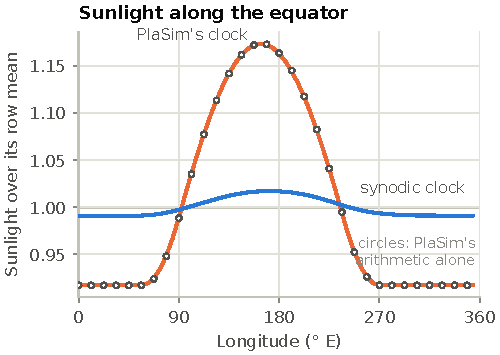
\includegraphics[width=0.6\textwidth]{figures/fig_sun_clock.pdf}
\caption{Sunlight at the top of the air along the equator, by longitude, over its row mean. Under PlaSim's
own Sun clock (run \code{A28\_dim5}, years 15--24) the Sun sweeps 392.5\textdegree\ each model day and skips
back 32.5\textdegree, leaving 270--57\textdegree~E 8.3\% short and the far side up to 17\% over; the circles
rebuild that pattern from PlaSim's solar-position arithmetic alone. Under the synodic clock
(\code{A28\_dim5\_sun\_test}) the row varies only by the 0.991--1.017 that 12.1 lunar days in a model year
give.}
\label{fig:sunclock}
\end{figure}

\textbf{Defects of the adaptation.} The adaptation made defects of its own, found some by checks of the
kinds set out under Verification and some in the course of the work. The GCM runner first extended the solar
spectrum past its 2.73~\textmu m end at its last value, an invented infrared tail that put 86\% of the
sunlight in the near infrared and warmed the first run past 320~K.\claim{H28} The first electrified build
discharged once per 6~s step, after all the step's charging, so the field stood a median 3.2 times breakdown
at a step's first discharge, which removed a median 150~C. Its fall-speed scaling multiplied memory the
scheme had left unset, and an OpenMP directive made private a variable the threads shared, both caught when
results changed with the thread count; and the first lunar gravity patch scaled the NSSL fall speeds and
missed the ventilation tied to them, so lunar rain evaporated 1.3--1.5 times too fast for its size until a
code review found it.\claim{H29} The sky model's 114 production channels averaged optical depth over windows
and opaque lines and absorbed 58\% too much sunlight above 500~nm with the Sun overhead, which had made
PlaSim look short of its calibration; the curved-air ledger's first channels, bisected on the whole column
alone, put near-infrared sunlight too high, 19.0 against 10.7~W\,m$^{-2}$ at 66--85~km, and the first two
20-year GCM tests of the curved air ran on those terms.\claim{H30} The first terrain build placed its forcing
by a corner column standing 2.9~km up. CM1's starting soundings held the GCM's top-level vapour constant above
the GCM's 130~km top, 6--15 times saturated over ice at 140--150~km in the 45\textdegree\,N rings, and the
45\textdegree\,N twilight pair ran its two halves on builds compiled at different optimisation
levels.\claim{H31} The last two remain in the runs made before they were found.

\textbf{What a slice of the GCM lacks.} Running CM1 inside the GCM's climate adds a structural limit to
the inherited ones. A ring of columns along a latitude circle misses the transport across the circle, a
box misses any day--night circulation larger than itself, and stock CM1 needs three things added: a lunar
Sun, forcing above its boundary layer and nudging that follows terrain. Two of these absences showed in
runs. The first box, forced with the advection along the rings alone, rained in the mornings and stayed
clear and hot in the afternoons until it was stopped at day 47, and at 45\textdegree\,N the missing
transport across the circle accounts for about a third of CM1's warm offset from the GCM.\claim{H32} The
forcing methods that answer these limits borrow from the GCM whatever the slice lacks, and so inherit the
GCM's remaining Earth.

\begin{table}[p]
\caption{The inventory of hidden Earth on the paths the lunar runs use, at Terluna commit 186b294. Form: a
constant, a unit of time, geometry, a fit or simplification used beyond its range (Fit), or a defect. State: a
general repair; a general method with a lunar table; a calibration to the lunar design case; a setting of
the lunar scenario; a capability added; a bound; avoided by configuration; bypassed; mitigated; or open.
Opt-in repairs are off in the design case.}
\label{tab:inventory}
\footnotesize
\setlength{\tabcolsep}{4pt}
\renewcommand{\arraystretch}{1.08}
\begin{tabularx}{\textwidth}{@{}>{\raggedright\arraybackslash}p{0.15\textwidth}LL>{\raggedright\arraybackslash}p{0.085\textwidth}>{\raggedright\arraybackslash}p{0.125\textwidth}@{}}
\toprule
Part & Earth in the code & On the Moon & Form & State \\
\midrule
\multicolumn{5}{@{}l}{\textit{ExoPlaSim 3.4.2 (PlaSim)}} \\
Sun clock & Restarts each model day & Skips back 32.5\textdegree\ a day & Defect & General \\
Orbit default & Earth's orbit for 1~AD & Tilt 23.7\textdegree\ for 1.54\textdegree & Defect & General \\
Calendar & 360-day year of 17,280 steps & Output slips 120 steps a year & Time & General \\
Convective cover & Rain per model day & Cover $+0.42$ & Time & General \\
Cloud water & CCM3 height scale in metres & Cloud above 20~km nearly dry & Constant & General \\
Slant path & Horizon factor 35 & 13.5 for water, 7.1 for air & Geometry & Method, lunar table \\
Columns & Flat, lit with the Sun up & Miss a net 5.8~W\,m$^{-2}$ loss & Geometry & Method, lunar table \\
Shortwave gases & Omit CO$_2$ and O$_2$ & Their share taken by water & Fit & Calibration \\
Rayleigh, continuum & 5772~K normalisation; continuum 0.024 & First design run past 310~K & Fit & Calibration \\
Water absorptivity & Lacis--Hansen, Earth's paths & Air 7.7--8.2 points short & Fit & Calibration \\
Longwave by height & Sasamori's absorptivities & Lowest layers overcooled 10--12~W\,m$^{-2}$ & Fit & Calibration, opt-in \\
Cloud phase & Liquid optics for all cloud & Ice cloud at 165--204~K & Fit & General, opt-in \\
Saturation & Over liquid; Earth's top levels & Cloud at 136--149\% of ice saturation & Fit & Open \\
Lowest level & Probably the spectral transform & Up to 20~K cold in 0.8\% of windows & Defect & Open, screened \\
Dynamics & Constant $g$, thin shell & $g$ 5.4\% lower at 48.6~km & Geometry & Open \\
\midrule
\multicolumn{5}{@{}l}{\textit{CM1 release 22}} \\
Gravity & 9.81 in four routines on the lunar paths; fall speeds & Fall speeds 2.3--6 times too fast & Constant & General \\
Rain size & Mean under 2.8~mm; breakup from 0.3~mm & Stable drops 2.46 times larger & Fit & Open \\
RRTMG gases & CO$_2$ by year; Earth's trace gases & Earth's air & Constant & Setting \\
RRTMG pressures & Tables from 1,053.63~hPa & Lowest 7.5~km extrapolated & Fit & Open \\
RRTMG ice & Optics to 140~\textmu m & Crash at day 6.45 & Fit & Mitigated \\
RRTMG Sun & Unfiltered spectrum & 5~W\,m$^{-2}$ of clear-air absorption & Constant & Open \\
Day & Earth's Sun and calendar; soil 1--16~cm & Thermal wave 0.6~m deep & Time & General (Sun); setting (soil) \\
Damping, mixing length & 300~s; 75~m & Earth's scales & Constant & General \\
Beta plane & Earth's rotation and radius & Earth's $\beta$ & Constant & Bypassed \\
Threads & Unlocated race & Runs on several threads part & Defect & Open \\
\midrule
\multicolumn{5}{@{}l}{\textit{WRF-ELEC, grafted into CM1}} \\
Gravity, ventilation & 9.8; fall speeds; ventilation & Fall speeds Earth's; scaled alone, rain evaporates 1.3--1.5 times too fast & Constant & General \\
Breakdown cap & 180~kV\,m$^{-1}$ & Binds below 36~km & Constant & General \\
Ground strike & $-7$\,\textdegree C level; stopping field 0.15 & Level 27--34~km up & Constant & Bound \\
Sub-step & 0.75~s for 500~m layers & 2~km layers, slow graupel & Constant & General \\
Flash reach & Logged above a charge threshold & Weak high flashes logged none & Constant & General (logging) \\
Conduction & None in clear air & Charge persists for weeks & Time & Capability \\
Charging, thresholds & Laboratory laws; 50~MV, 10~kV\,m$^{-1}$ & Polarity turns with the law & Fit & Open \\
\midrule
\multicolumn{5}{@{}l}{\textit{SWAN 41.51 and SWASH 12.01}} \\
Wind-input knee & 1~Hz & Similarity off by 5.44\% & Constant & General \\
Air density & 1.28~kg\,m$^{-3}$ & About 1.40~kg\,m$^{-3}$ & Constant & Setting \\
Breaker parameter & Read uninitialised with breaking off & Repeats differ by 2.5\% & Defect & Avoided \\
Other defaults & 2~s initial period; $g$ in ST6, XNL; Earth's radius, rotation & Earth's values & Constant & Avoided \\
Empirical laws & Wu, Komen, AGROW, breaker 0.73, breaking 0.6 and 0.3 & Uncalibrated & Fit & Open \\
\bottomrule
\end{tabularx}
\end{table}

\section{Repairs}

Most repairs follow one rule: an Earth value or a defect becomes a parameter whose default reproduces the
released code, so that the repair can be switched off and its effect compared with the original. Some
changes depart from the rule, and Table~\ref{tab:repairs} marks them. CM1's deeper soil and its zeroed trace
gases and ozone act in every patched build; its 400~ppm default for carbon dioxide replaces the calendar
formula, and the electrified build's gravity defaults to 9.81 where the released NSSL scheme has 9.8; the
beta plane's Coriolis force acts on departures from the base-state wind in beta-plane runs; the electrified
build caps the ice sizes its radiation reads; and SWAN's air density is compiled in. SWAN's wind-input patch
reproduces stock output only at standard gravity, 9.80665~m\,s$^{-2}$, set by input, and the guard added to
the water scaling is the identity only for spectra like the design case's. Each change is recorded as a patch
against a pinned upstream source, with its switch, its default and the checks made on it.

Three classes of repair differ in where their lunar values come from. A general repair corrects a unit,
applies a scaling law or a physical law, or removes a defect; its value follows from physics or from the
code's own intent, and another world takes it unchanged within the limits of Table~\ref{tab:reach}. A
general method with a per-world table computes a quantity of a world's own column, a path ratio or an energy
difference, and tabulates it, so the method serves another world once its table is computed there. A
calibration adjusts the free coefficients of an approximate scheme until its output matches the reference
model on chosen columns, and holds near the states it was fitted on. The line between the last two lies in
the tuning: the curved-air terms follow from the column's geometry and its computed radiation, while the
coefficients of the gas bands were fitted until PlaSim matched the line-by-line model's absorption. Beside
the three classes stand settings, which give the scenario's values; capabilities, which add a process or a
forcing the released codes lack; a bound, where the physics is unsettled; a mitigation; avoidances by
configuration; and a coupling method.

\textbf{Defects removed or avoided.} Patch 04 turns ExoPlaSim's Sun at the synodic rate continuously from the
first step, a mode that assumes a steady, non-synchronous rotation and counts the Sun's phase from step 0.
Patch 03 converts convective rain per 86,400~s. ExoPlaSim's own \code{fixedorbit} switch, whose documentation
describes only the freezing of Milankovitch variations, holds the configured orbit, and a year of 17,160
half-hour steps, twelve whole lunar model days, keeps output aligned with the Sun. SWAN's breaker parameter
is avoided by keeping depth-induced breaking on in every run, and SWAN's default initial state, whose 2~s
peak period has Earth's dimensions, by starting from rest or from hotstart files. The thread race and PlaSim's
cold lowest level stay open: CM1 runs that must repeat use one thread, and analyses of the lowest level
screen the cold windows.

\textbf{Constants to parameters.} The ExoPlaSim repairs are ten patches to PlaSim's radiation, cloud and Sun
code, each adding a namelist switch whose default is the released behaviour. In CM1, gravity and the air's
carbon dioxide and oxygen become preprocessor constants that default to 9.81~m\,s$^{-2}$, 400~ppm and
Earth's oxygen, and CM1's twenty spare namelist reals hold the lunar Sun, the forcing and the
electrification's settings. SWAN's wind-input knee moves with gravity and stays at 1~Hz under standard
gravity. The lunar runs were made with runners, the scripts that configure, compile and run each model, which
insert each change into the installed source at a marked anchor. The code repository holds the changes as
patch series against pinned upstream archives, and a script rebuilds from those archives, byte for byte,
the deployed ExoPlaSim installation and the Fortran of the eight lunar CM1 builds used for the results
reported here, while older CM1 builds, the Earth-gravity benchmark builds among them, were compiled from
earlier states of the series.\claim{R01}

\textbf{Scaling laws.} Where gravity enters a fitted law, a similarity argument gives the repair. A particle
falling in the regime $V = aD^b$ has a Reynolds number that grows as the Best number to the power
$(b+1)/3$ \autocite{mitchell1996use}, and the Best number of a particle of fixed size is proportional to
$g$, so $V \propto g^{(b+1)/3}$: at lunar gravity cloud droplets fall 6.04 times slower, raindrops 2.94 times
and graupel 2.27 times.\claim{R02} The scaling is exact for particles whose mass grows as $D^3$ and area as
$D^2$, as for drops, graupel and hail, within their fitted regimes; snow and ice crystals, whose mass and area
follow other powers, take a larger gravity exponent than the patch gives them. The Morrison and NSSL schemes
pass the scaled speeds through their fall-speed laws and caps into collection and ventilation, and in NSSL
the ventilation needed its own scaling at eleven sites.

The same argument sets other lengths and times. CM1's Rayleigh damping rate and its boundary-layer length
scale as $g$ and $1/g$, as the dynamics stretch, and WRF-ELEC's sub-step lengthens from 0.75 to 6.8~s, which
keeps graupel settling through about 1\% of a layer per sub-step in the 2~km layers of the lunar charging
zone, at 0.44 of Earth's fall speed; the boxes, rounding to whole sub-steps, run one 8~s sub-step per model
step.\claim{R03} The breakdown field already scales with the air's density, and lifting its
180~kV\,m$^{-1}$ cap lets that scaling act wherever lunar flashes start. SWAN's knee becomes a function of
$f\,g_\mathrm{E}/g$, which reproduces stock SWAN at standard gravity and restores the model's gravity
similarity.\claim{R04} The repairs of units and heights restore the quantity each formula was written for.
CCM3's cloud water counts heights and precipitable water at Earth's gravity and scales its mixing ratio by
$g/g_\mathrm{E}$, which gives each cloud the water path it would hold at the same pressures on Earth, and
CM1's five soil layers thicken to 5--80~cm, 1.55~m in all, deep enough for the thermal wave of any solar day
from a few Earth days to the Moon's.

\textbf{Geometry restored.} The curved geometry enters both models through an energy ledger of the design
column: the radiation of the same air traced once, offline, through spherical shells and through flat layers,
and the differences tabulated. For the ledger, sunlight from 360~nm to 5~\textmu m was traced through 100
spherical shells and through the same layers taken flat, at solar elevations from $-90$ to 90\textdegree, in
10,697 spectral channels. Each channel absorbs a direct beam within 1\% of its sunlight as its members do and,
beyond 1,250~nm, keeps the beam's loss above every layer; below 500~nm each band is one channel. The 282
channels below 1,250~nm thin enough to scatter take spherical successive orders of scattering from an in-house
sky solver, and the rest a direct beam through the shells with the diffuse light of a pseudo-spherical
two-stream, so their twilight lacks scattered light. The infrared escape is traced through the same shells by
impact parameter. The ledger's terms divide the curved geometry into the widening of the shells above each
square metre of ground, worth $-6.5$~W\,m$^{-2}$ net, and the curved light and escape, the twilight and the
low Sun's side light, worth $+0.7$~W\,m$^{-2}$.\claim{R05} Tabulated at 167 solar elevations from $-40$ to
90\textdegree, the terms add sunlight to each PlaSim layer or CM1 shell and the ground's share in the column's
clear share, below the horizon as well as above, and remove each layer's extra infrared escape, scaled with
temperature to the fourth power. PlaSim's slant factor becomes the Moon's, $(\mu+a)/(\mu^2+b\mu+c)$ fitted to
straight rays through the shells, within 0.30\% for water vapour and 0.08\% for well-mixed air
(Figure~\ref{fig:slant}).\claim{R06} Part of the daylight term is a difference of solvers: with the Sun
overhead, where the geometry is flat, the spherical solver's ground still takes 1.3\% less than the
two-stream's, so the daytime term also corrects the reference column PlaSim was calibrated against.\claim{R07}

\begin{figure}[tbp]
\centering
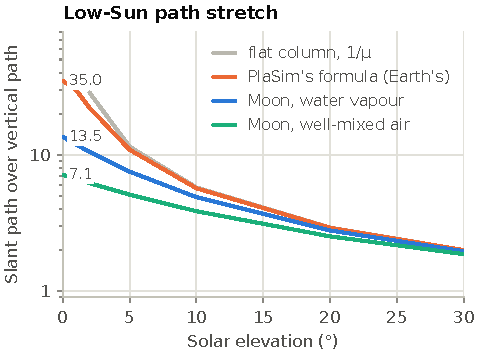
\includegraphics[width=0.6\textwidth]{figures/fig_slant.pdf}
\caption{The slant path over the vertical path as the Sun nears the horizon. PlaSim's formula,
$35/\sqrt{1+1224\mu^2}$, has Earth's horizon value; the Moon's factors for water vapour and for well-mixed
air come from straight rays through the design column's shells. The flat column's $1/\mu$ diverges at the
horizon.}
\label{fig:slant}
\end{figure}

\textbf{Calibration by height.} PlaSim was calibrated against the in-house radiative--convective model and
its correlated-$k$ emulation. The model is clear-sky and line-by-line, built on HITRAN lines of water, carbon
dioxide and oxygen as served in September 2026 (HITRAN2020 or a later edition), a re-implementation of
MT\_CKD~4.3, collision-induced absorption and Rayleigh scattering, with gravity falling as $GM/r^2$ and a
pseudo-spherical direct beam; its emulation reproduces the outgoing longwave within 0.4~W\,m$^{-2}$ at
288--290~K and within 1.4~W\,m$^{-2}$ for a saturated 330~K lunar column.\claim{R08} Each calibration was made
to remove the residual of the one before. The first fitted two totals, a Rayleigh multiplier and a weaker
water continuum on global-mean columns, which brought the clear-sky albedo within 0.007 and the outgoing
longwave within about 2~W\,m$^{-2}$. Once the Sun-clock and orbit defects were found, a check of how each
column split its own arriving sunlight showed the air 7.7--8.2 points short, and a multiplier on the
near-infrared water absorptivity, refitted with the Rayleigh multiplier on eleven columns, brought the split
within 0.3 points rms.\claim{R09} By layer the fit still placed sunlight low: PlaSim put almost nothing above
85~km, where the line-by-line column absorbs 4.2~W\,m$^{-2}$. Three carbon dioxide and oxygen bands, each
fitted to the line-by-line beam's loss above every level within 0.13\% of its energy, and a refit of both
multipliers brought the layers within 0.97~W\,m$^{-2}$ rms of the reference, from 1.71
(Figure~\ref{fig:layers}).\claim{R10} In the longwave, a fit to totals proved insufficient: PlaSim's water
continuum had been fitted to the outgoing flux, which a scheme can match while misplacing its cooling by
10~W\,m$^{-2}$ in a layer. An extra escape to space for each layer and for the ground, fitted over land and
over sea on about 2,100 cloud-free three-day means and scaled with temperature to the fourth power, removes
each layer's mean error and leaves 1--5~W\,m$^{-2}$ from column to column.\claim{R11}

\begin{figure}[tbp]
\centering
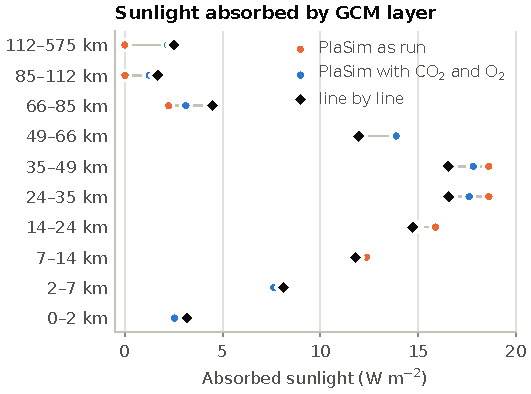
\includegraphics[width=0.62\textwidth]{figures/fig_layers.pdf}
\caption{Sunlight absorbed in each GCM layer of the design column, global means: the line-by-line
pseudo-spherical model against PlaSim's arithmetic on the same column as run, and with the carbon dioxide
and oxygen bands and the refitted multipliers. With the bands the layers come within 0.97~W\,m$^{-2}$ rms of
the reference, against 1.71 as run; about 2~W\,m$^{-2}$ of water's sunlight still lands at 35--66~km in
place of 66--85~km and the lowest 7~km.}
\label{fig:layers}
\end{figure}

\textbf{Processes and capabilities added.} Cloud colder than $-38$\,\textdegree C takes Ebert and Curry's ice
optics \autocite{ebert1992parameterization} through a delta-scaled two-stream, with an effective radius from
Kristjánsson and Mitchell's table \autocite{kristjansson2000impact}, in place of liquid water's, a physical
law in place of a simplification. WRF-ELEC's charge separation, discharge and screening, which CM1 lacks,
were grafted into it: the NSSL scheme with charge on every hydrometeor; a Poisson solver by Fourier transform
across the periodic domain and a tridiagonal solve on CM1's stretched levels; WRF-ELEC's cylindrical
discharge \autocite{ziegler1994observed} and its three-dimensional discharge adapted from
\textcite{macgorman2001lightning}, on a domain that wraps round; and its screening layers, available and off
in the lunar runs.\claim{R12} The lunar runs add leakage of charge through a computed lunar conductivity
column, and a leader's crossing to the ground at an internal field of 1~kV\,m$^{-1}$ at sea-level density,
scaled with the air's density, which places the ground strikes between the bounds set by WRF-ELEC's stopping
field and its $-7$\,\textdegree C rule; point discharge from the ground, added as an option, ran in one test
window and stays off.\claim{R13} PlaSim gains a downward infrared flux at the model top, by day and by night,
for any source above the air, a host planet's glow for a moon among them, and CM1's radiation reads ice sizes
capped at RRTMG's 140~\textmu m, with the excess logged.

\textbf{Forcing a slice of the GCM.} Running CM1 inside the GCM's climate adds a structural limit to the
inherited ones: a ring of columns along a latitude circle lacks the transport across the circle, a box lacks
any day--night circulation larger than itself, and stock CM1 has no lunar Sun, no forcing above its
boundary layer and no nudging that follows terrain. Two of these absences showed in the runs. The first box,
forced with the advection along the rings alone, rained in the mornings and stayed clear and hot in the
afternoons until it was stopped at day 47, and at 45\textdegree\,N the missing transport across the circle
accounts for about a third of CM1's warm offset from the GCM.\claim{H32} The forcing methods supply what the
slice lacks from the GCM's fields, and with them the GCM's remaining Earth values. Each ring column has its own
Sun (a box takes one) and, on tilted rings, its own Coriolis parameter; CM1 is nudged toward the GCM only above
8--16~km, so its boundary layer and convection develop freely, and the GCM's mean vertical wind enters CM1's
own large-scale advection.\claim{R14} A heating and moistening by local time and height supplies the
day--night circulation a box lacks and, as a single local-time bin, the transport across the circle a ring
lacks; over terrain each column is nudged and forced at its own height above sea level. SWAN takes the GCM's
surface stress through Wu's drag law inverted to an equivalent wind, so its friction velocity matches the
GCM's to within a few per cent, on spherical coordinates at the lunar radius and with its frequency band
scaled by $g/g_\mathrm{E}$; SWASH, unmodified, takes lunar gravity as an input and SWAN's spectra at its
boundary.\claim{R15}

\section{Verification}

Six kinds of check were made, each testing something further from the code than the one before
(Table~\ref{tab:verification}). Identity and reproduction checks test the code alone: a patch at its default
leaves the arithmetic of the build without it unchanged along the trajectory tested, and the recorded code and
results can be rebuilt. Arithmetic checks test an implementation against a formula or a direct solution. A
similarity check tests whether gravity enters the code consistently, by showing that a run at scaled gravity,
lengths and times reproduces the original in dimensionless form. Calibrations and benchmarks compare with
something outside the code: the reference model on the columns a fit was made on, and a scheme's published
behaviour on Earth. Each leaves the lunar climate untested in its own way, since the reference is itself a
clear-sky model resting on its spectroscopy, a fit holds near its fitted state, similarity leaves Earth's
empirical laws untested at lunar gravity, and a benchmark runs on Earth.

\textbf{Identity and reproduction.} Five ExoPlaSim runs, each a model year from one restart, repeat byte for
byte the restart file of the same build without the patch, with the patch at its neutral setting: the
Rayleigh and continuum calibration at the released values, the cloud-water and convective-day patches,
infrared from space at zero, and the ice optics off. One of them compares against the released model itself,
and the other four against builds that already had earlier patches, so the chain back to the release closes
through those patches' own identities; a year killed a minute in and resumed repeats the uninterrupted year's
restart and every variable of its output.\claim{V01} In CM1 the tilted-ring patches and the local-time
advection repeat an existing run's first model day bit for bit, single-thread runs repeat, and the electrified
supercell, restarted on four threads and on two, repeats its fields and its 41 flashes; SWAN with the
wind-input patch writes stock output at standard gravity.\claim{V02} Applied to the pinned upstream archives,
the patch series rebuild byte for byte the deployed ExoPlaSim installation and the Fortran of the eight lunar
CM1 builds used for the results, and prefixes of the ExoPlaSim series reproduce the source hashes of 32 of
the 34 GCM runs that recorded one.\claim{V03} The Sun clock, the water scaling, and the curved-air, gas-band
and longwave patches (07--09) were written to reproduce the released code at their off settings, and have yet
to be run that way.

\textbf{Similarity.} The strongest evidence about gravity comes from the similarity checks. Stock SWAN, run at
a sixth of Earth's gravity with lengths, depths and durations six times longer and frequencies six times
lower, misses its Earth twin by 5.44\% in significant wave height and 3.91\% in mean period; patched, it misses
by 0.303\% and 0.326\%, against a 1\% criterion.\claim{V04} SWASH reproduces the linear dispersion relation
within 1.76\% in amplitude and 0.289\% in phase at lunar, four times lunar and Earth gravity, preserves a linear
waveform to 0.0009\% of its amplitude when gravity quadruples and the clock halves, and, under the same scaling
with breaking and a moving shoreline, changes its 98th-percentile run-up by 1.20\%.\claim{V05} Each lunar wave
run is therefore the gravity-scaled image of an Earth run with the same Earth-fitted coefficients, and whether
those coefficients hold on lunar seas is untested. CM1's gravity-scaled microphysics has no such test yet:
the pair of runs designed to measure how far lunar convection departs from Earth's stretched sixfold failed to
convect.\claim{V06}

\textbf{Calibration and the reference.} The calibrations hold on the columns they were fitted to and a little
beyond. The clear-sky split of sunlight holds within 0.6 points rms on eleven columns outside the fit's set,
and a 303~K column carrying 338~kg\,m$^{-2}$ of vapour, warmer and wetter than any fitted, falls 0.7 points
short, where the scheme before its water recalibration fell 9.7 short.\claim{V07} RRTMG, checked and left
uncalibrated, lies within 2.5 points of the line-by-line shares of reflected, air-absorbed and ground-absorbed
sunlight at the site where the rings cross the equator at 0\textdegree~E, and on 990 cloud-free columns of the
45\textdegree\,N ring cools the air more than the correlated-$k$ model does, by 4.5~W\,m$^{-2}$ in the lowest
1.8~km, 8.5 at 1.8--6.5~km and 10.2 at 6.5--13.7~km.\claim{V08} Every calibration is clear-sky, and PlaSim's
clouds remain uncalibrated. The accuracy of all of them is bounded by the reference's own. Its correlated-$k$
emulation reproduces the line-by-line outgoing longwave within 0.4--1.4~W\,m$^{-2}$, and the line-by-line
model has two checks against other codes: PyRADS, for longwave with water vapour alone at constant gravity,
and a Monte Carlo reference for Rayleigh scattering up to an optical depth of 1.5, where the lunar column
reaches about 4 at 360~nm. No independent code has yet checked its carbon dioxide, oxygen, collision-induced
absorption or sunlight on the lunar column.\claim{V16}

\textbf{Benchmarks and arithmetic.} The electrified graft was benchmarked on Earth. Against CM1's own NSSL
scheme in the Weisman--Klemp supercell \autocite{weisman1982dependence}, its largest updrafts stay within 6\%,
its reflectivity within 3.4~dBZ at every half hour and its condensate within 9\%, while hail differs by up to
a factor of two, the two copies being different versions of the scheme.\claim{V09} Against published runs of
the same charging and lightning schemes, the first flash comes at 28.5 minutes against a published 27--40, and
the flash rates and the median charge per flash fall within the published ranges; with WRF-ELEC's ground rule
on, 1.1\% of flashes struck the ground, against 0.33\% in a published run. The charging runs several times
stronger, traced to cloud ice reaching $2\times10^8$ crystals per kilogram where droplets freeze homogeneously
in 50~m\,s$^{-1}$ updrafts.\claim{V10} The lunar conductivity column reproduces Earth's measured fair-weather
positive conductivity within 2--8\% from 5 to 30~km at a 3~GV cutoff. Arithmetic checks rebuild the uneven
sunlight of the Sun-clock defect from PlaSim's solar-position arithmetic with correlation 1.0000, place a
tilted ring's Sun within $8\times10^{-7}$ of the spherical formula and its Coriolis parameter within
$3\times10^{-12}$~s$^{-1}$ of $2\Omega\sin\phi$, match the field solver to a direct solve to one part in
$10^5$, and hold the curved-air ledger's channels within 0.9~W\,m$^{-2}$ of the fine spectral grid in every
layer with the Sun overhead.\claim{V11}

\textbf{What the checks caught.} The adaptation introduced defects of its own, found by these checks or in
the course of the work. The GCM runner first extended the solar spectrum past its 2.73~\textmu m end at its
last value, an invented infrared tail that put 86\% of the sunlight in the near infrared and warmed the first
run past 320~K.\claim{H28} The first electrified build discharged once per 6~s step, after all the step's
charging, so the field stood a median 3.2 times breakdown at a step's first discharge, which then removed a
median 150~C. Its fall-speed scaling multiplied memory the scheme had left unset, and an OpenMP directive made
private a variable the threads shared, both caught when results changed with the thread count; and the first
lunar gravity patch scaled the NSSL fall speeds but left the ventilation tied to them at Earth's values, so
lunar rain evaporated 1.3--1.5 times too fast for its size until a code review found the omission.\claim{H29}
The spherical sky solver's production grid of 114 spectral channels averaged optical depth over windows and
opaque lines and absorbed 58\% too much sunlight above 500~nm with the Sun overhead, which had made PlaSim look
short of its calibration; the ledger's first channels, bisected on the whole column alone, put near-infrared
sunlight too high, 19.0 against 10.7~W\,m$^{-2}$ at 66--85~km, and the first two 20-year GCM tests of the
curved air ran on those terms.\claim{H30} The first terrain build placed its forcing by a corner column
standing 2.9~km up; CM1's starting soundings held the vapour of the GCM's top level, near 130~km, constant
above it, so the 45\textdegree\,N rings began 6--15 times saturated over ice at 140--150~km and every column
kept 1.1~g\,m$^{-2}$ of ice above 107~km through both lunar days; and the 45\textdegree\,N rings with and
without the curved-air terms, the twilight pair, ran on builds compiled at different optimisation levels, so
their 0.013--0.021~K difference lies below what the pair resolves.\claim{H31} The last two remain in the runs
made before they were found.

\textbf{Checks that fell short.} SWAN with depth breaking off failed its repeatability test by about 2.5\%, and
tracing the failure found the uninitialised breaker parameter. SWAN's early growth depends on the time step:
halving it changes the first hours' wave height by up to 33\%, while the 48-hour endpoints move under 0.3\%,
and small seas in the weather runs fail their 5\% time-step criterion where seas above 1~m pass. SWASH's control
with irregular input misses its 5\% bound, at 5.22\% in height and 6.28\% in period.\claim{V12} CM1 rebuilt at a
higher optimisation departs from its first build by 0.28--0.32~\textdegree C rms in the air at 2~m within a
model day, inside the spread of last-bit nudges, and on several threads it departs from itself. The ledger's
scattering orders reached their cap in one channel of 282, whose omitted tail is about $3\times10^{-4}$ of that
channel's diffuse light at the ground.\claim{V13}

\textbf{Checks still to make.} The full design column has yet to be run through an independent radiation code
with every absorber, which would test the reference on which all the calibrations rest. CM1 has yet to be
forced from the longwave-corrected GCM, so whether the corrected physics closes the gap between the two
models is untested. The longwave correction, fitted at 295~K, ran in a test that settled near 307~K with twice
the water vapour, and its accuracy there is unchecked. The twilight pair lacks a control on the same build and
an estimate of its realisation noise. CM1's thread race remains unlocated, RRTMG's extrapolation past its
tables and CM1's gravity-scaled microphysics remain untested on their own, and an independent GCM has yet to
run the scenario.\claim{V14}

\section{What the adapted models have given}

The repaired models are instruments for the lunar climate, and their first products are sensitivities: how
far each Earth assumption, once removed, moves the climate, and where the uncertainty that remains now sits.
Every climate number below is a conditional model result, holding given the scenario and the Earth-fitted
parts each model keeps.

\textbf{What each repair moved.} Figure~\ref{fig:repairs} sets each repair's effect on the global-mean
surface temperature beside the sensitivity tests, each pair of runs averaged over set years and several
still drifting. On the first design run, with 25\% seas under the undimmed shield, counting cloud water by
pressure warmed the Moon by 2.3~K over the years averaged and about 2.5~K as the run settled, and counting
convective rain per Earth day warmed it by a further 1.8~K, about 1.6~K settled.\claim{G01} The Sun clock,
the Moon's own tilt and the recalibrated split of sunlight warmed it by only 0.6~K, yet cut its rain from
2.91 to 2.24~mm per day and raised the share of land receiving under 0.5~mm per day from 9 to
42\%.\claim{G02} The curved air cooled it by 0.65~K, its clouds giving back in the first year 3.5 of the
5.4~W\,m$^{-2}$ that the geometry took from the clear sky, and the carbon dioxide and oxygen bands cooled it
by a further 2.2~K, mostly through PlaSim's high cloud, since a cloud-free column moves its ground only
0.57~K: the high deck fell from 16 to 12\% of the sky, the top layer's cirrus from 2.0 to 0.05\% as that
layer warmed by 7~K.\claim{G03} Held at the design temperature by dimming the sunlight 3.0\% in place of the
earlier 5\%, the corrected Moon settles at 295.0~K, with 2.31~mm of rain a day.\claim{G04}

\begin{figure}[tbp]
\centering
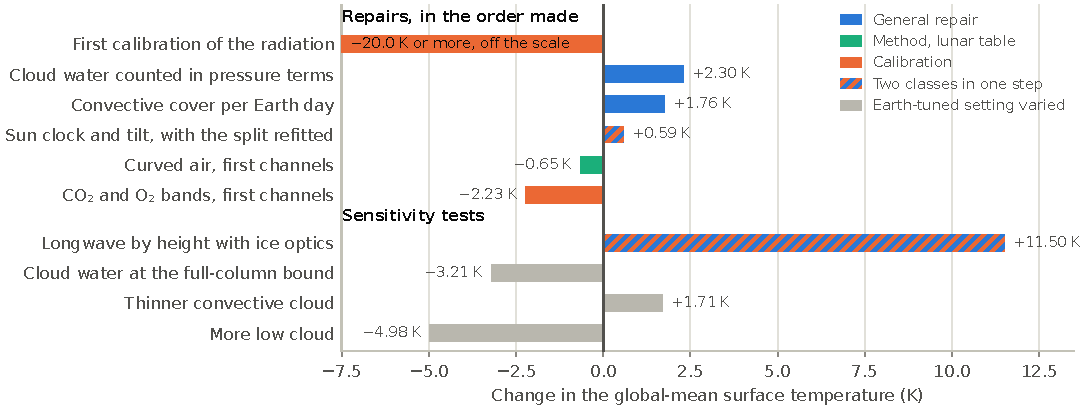
\includegraphics[width=\textwidth]{figures/fig_repairs.pdf}
\caption{Change in the global-mean surface temperature from each repair in the design case and from four
sensitivity tests, each against its own baseline: run A (25\% seas, the undimmed shield) for the cloud
water, the convective cover and the full-column bound; the design run before and after the Sun and tilt
repairs for those; the corrected run of 2026-09-29 for the curved air and the two cloud settings; the
curved-air run for the gas bands; and the current design case for the longwave test. Bars are means over the years given in the
accompanying data, against each baseline's own years; several runs were still drifting, and the longwave
test extrapolates to balance at 306.8--307.1~K.\claim{G13}}
\label{fig:repairs}
\end{figure}

The climate is most sensitive where the models remain Earth's. Two of PlaSim's Earth-tuned cloud settings
move the Moon as far as the repairs do: thinner convective cloud warms it by about 2.2~K and more low cloud
cools it by about 5.9~K as the runs settle, farther than any repair, and cloud water at its full-column
bound cools run A's Moon by about 3.5~K. The longwave correction with the ice optics, the one change that
moves the cooling by height, warms the Moon by 11.5~K over years 10--19, toward a balance near 307~K with
twice the water vapour, 348 against 170~kg\,m$^{-2}$, and cloud over 38\% of the sky in place of 20\%, most
of the gain high.\claim{G05} Cloud amount and the vertical placement of the longwave cooling therefore carry
the lunar climate's largest open uncertainty, and both rest on fits that cloud-resolving runs, the reference
model and an independent GCM can constrain.

\textbf{The gap between the models.} The cloud-resolving model and the GCM disagree near the ground, and the
forcing methods let the disagreement be taken apart. On the 45\textdegree\,N ring the lowest 1.8~km of CM1
ran 5.9~K warmer than the GCM over the second lunar day; imposing the GCM's transport across the circle,
about 15~W\,m$^{-2}$ of heat carried out of the air below 8~km, cut the offset to 3.7~K
(Figure~\ref{fig:gap}).\claim{G06} PlaSim's longwave over-cooling of its own lowest layers accounts for
about 1.5~K of the rest, and the remainder, a degree or two, is attributed by elimination to how the two
models carry the ground's heat upward, CM1 mixing its lower air 14--19~km deep by day where the GCM's stays
stable. At the equatorial crossing, on the GCM's forcing before its corrections, three other suspects were
tested and cleared: a three-dimensional box ran warmer still, the land surface moved the air by at most
0.3~\textdegree C, and rain falling at Earth's speeds warmed the air by a further 1.0~\textdegree C; at
45\textdegree\,N the dry-ground land test has yet to run.\claim{G07} Rain shows the larger disagreement. On
the GCM's forcing before its corrections, a small box brought 34~mm to the ground per lunar day where the
GCM that forced it rained 129~mm, and the corrected GCM 180~mm; at lunar gravity 85\% of the water falling
from the box's clouds evaporated on the way down, against 64\% when the same drops fell at Earth's
speeds.\claim{G08}

\begin{figure}[tbp]
\centering
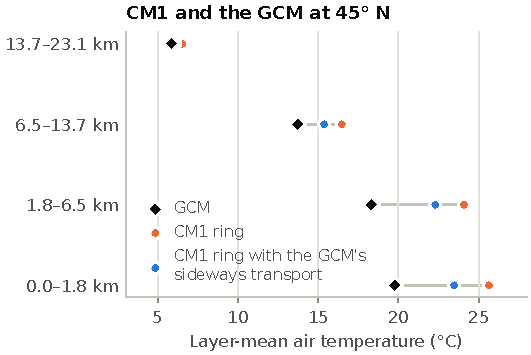
\includegraphics[width=0.62\textwidth]{figures/fig_gap.pdf}
\caption{Layer-mean air temperature over the second lunar day on the 45\textdegree\,N ring: CM1 alone, CM1
with the GCM's transport across the circle imposed, and the GCM's design case on the same row, years
10--19. The imposed transport removes 2.2 of the 5.9~K warm offset in the lowest 1.8~km, 37\%.}
\label{fig:gap}
\end{figure}

\textbf{Storms and lightning.} At lunar gravity the 0\,\textdegree C and $-40$\,\textdegree C levels stand
five to six times higher than in Earth's tropics, near 25 and 60~km, and cloud tops reach
55--80~km.\claim{G09} The lightning the storms make is rarer and larger than Earth's. The main electrified
run, two lunar days of a box at 0\textdegree~E forced from the GCM before its corrections, made 530
flashes, 0.022 per square kilometre per year, about a hundredth of Earth's average; up to a fifth were
negative ground strikes, counted under WRF-ELEC's rule with the leader's crossing, an upper bound, and none
was positive. Each ground strike lowered a median 149~C where Earth's lower 5--30~C, while in-cloud flashes
neutralised a median 108~C. The charge keeps Earth's arrangement at five to six times its height: flashes
start a median 35.8~km up, and the main negative charge sits at 40--42~km, at $-13$ to $-14$\,\textdegree C,
just above the $-7$\,\textdegree C level as on Earth. Hail, which rimes faster than the lunar graupel, does
87\% of the non-inductive charging.\claim{G10}

Two of the storm results hang on choices that measurement or theory could settle. Under Takahashi's charging
law \autocite{takahashi1978riming} in place of Saunders and Peck's \autocite{saunders1998laboratory} the
storms separate as much charge with their polarity inverted, so the lightning's sign rests on laboratory laws
that disagree on the sign rimed ice takes in the little cloud water of the lunar storms; and with the NSSL
microphysics in place of Morrison's the same box runs 1.0~\textdegree C warmer at 2~m and its night fog at the
ground covers 29\% of the box in place of 56\%, so the lunar night fog depends on the microphysics by about a
factor of two.\claim{G11}

\textbf{Seas.} Forced by sixty days of the GCM's surface stress, SWAN finds the light lunar winds raising
big, slow waves: the same wind, fetch and duration build waves 4--5 times as high as on Earth, with periods
five times as long. Over the nearside sea, 5.29 million~km$^2$, the mean significant wave height is 1.39~m,
68\% of area and time stands at or above 1~m, and the largest sea reaches 4.9~m with a 19.3~s mean period.
Lunar waves keep Earth's steepness and travel at 0.41 of the speed of an Earth wave of the same length.
SWASH runs them up today's steep slopes to a 98th-percentile run-up of 2.1~m on the exposed face of the
eastern Smythii headland.\claim{G12} These wave results rest on the corrected design climate as it stood
before the curved air and the gas bands, and on Earth's laws for wind input, whitecapping and breaking.

\textbf{What stays conditional.} The conditions under these numbers differ in weight. The design temperature
of 295~K is a target held by dimming the sunlight; the 307~K state of the longwave test is a sensitivity
resting on a correction used beyond its fit. The warmth and humidity of the air near the ground, the air
people would live in, stand best as a range between the models, 3.7~K wide in the lowest 1.8~km at
45\textdegree\,N with the GCM's transport imposed and against the GCM before its longwave correction. The
lunar rain depends on a convection scheme fitted to Earth in the GCM and on Earth's drop limits in CM1, the
lightning's polarity on a laboratory charging law, and the seas on Earth's wave physics carried to lunar
gravity by similarity.

\section{Reach to other worlds}

The results sort the adapted models' parts by how far they moved the Moon, and the classes of repair sort
the same parts by how far they travel. The general repairs, which another world takes unchanged, moved the
global mean by a few kelvin at most and moved where sunlight and rain fall; the calibrations and the
Earth-tuned cloud settings, which another world must remake, moved it most. The general repairs are the
synodic Sun clock, the fixed orbit and whole model days, convective cover per Earth day, cloud water by
pressure, gravity throughout CM1 with the fall-speed scaling, CM1's Sun for any day and its deeper soil, the
lifted breakdown cap and the scaled sub-step, SWAN's knee, and the ice optics. Leakage and the methods that
force a slice of a GCM travel with their inputs, a conductivity column or a GCM's fields, and the leader's
crossing travels as a bound set between two of WRF-ELEC's rules; the curved-air terms travel as a method whose
table is computed again for each column; and the calibrations, the Rayleigh and water multipliers, the water continuum, the longwave
correction and the gas-band fits, hold near the case they were fitted on. Another world therefore takes the
general repairs unchanged and needs its calibrations, its ledger and its settings made again, with tools
that come with the repairs: the reference model, the ledger and offline copies of PlaSim's
radiation.\claim{W01}

\textbf{The defects in other users' runs.} Three of ExoPlaSim's defects act well beyond the Moon. Its Sun
clock, in any non-synchronous run whose rotation differs from one day, skips back $1/(N-1)$ of a turn each
model day, where $N$ counts the planet's rotations in a 360-day year, rounded to a multiple of 12 and floored
at 12: about 1\textdegree\ near Earth's rotation, 2\textdegree\ at a two-day rotation, 10\textdegree\ at ten
days and 33\textdegree\ at any rotation slower than 20 days.\claim{W02} Its convective-cover unit adds
$0.125\ln(\text{day}/1\,\text{d})$ to the cover in any run whose model day differs from one Earth day,
synchronous runs included, since ExoPlaSim's synchronous mode fixes the Sun in the sky and keeps the model
day its rotation period sets: about $+0.23$ for TRAPPIST-1e's rotation of 6.1 days and $+0.31$ for Proxima
Centauri~b's 11.2 days. Its default orbit gives Earth's seasons to any run that sets an obliquity or an
eccentricity without fixing the orbit.\claim{W06}

\textbf{Where Earth values break.} Against the ratios of Figure~\ref{fig:regimes}, each Earth value fails
along its own direction. PlaSim's horizon factor of 35 is right only at Earth's scale height over radius; an
isothermal Chapman factor gives 22 for present Mars, 24.5 for Venus, 14 for Titan and 7.2 for the Moon, so the
slant path errs for each and most for the tallest air, while PlaSim's broadband fits, made near Earth's
column, meet columns ten times Earth's on Titan, a hundred times on Venus and seven times on the Moon.
Slingo's cover, with its unit repaired, remains a fit made on Earth's convection, and PlaSim's cloud
water, written in metres, errs at any gravity other than Earth's, too dry aloft under weaker gravity and too
wet under stronger.\claim{W02} Released CM1 fails at any gravity but Earth's, under any day but Earth's
24 hours, and in any air whose carbon dioxide differs from Earth's value for the calendar year; SWAN, in the
configuration used, loses gravity similarity through one constant. Taken model by model, the adapted CM1
runs storms in Earth-like air at any gravity on its Morrison and NSSL paths, SWAN and SWASH run water seas at
any gravity by similarity with Earth's empirical laws, and ExoPlaSim, bounded by its radiation fits and its
cloud, has the narrowest reach of the three. Table~\ref{tab:reach} sets out, property by property, where the
released models break, what the adaptations now reach and what lies beyond them. Of the found worlds in
Figure~\ref{fig:regimes}, only Earth lies within that reach; the rest of it lies among constructed worlds and
among exoplanets whose air is taken to be close to Earth's.

\textbf{Within reach as adapted.} The breathable Moon under other dimmings runs in all four models with the
repairs as they stand, as long as its columns stay near the fitted ones: the split of sunlight holds to 0.7
points on a 303~K column with 338~kg\,m$^{-2}$ of vapour, while the longwave correction's accuracy near 307~K
is unchecked. At 1.0~atm, a case yet to be run, or behind another shield that blocks the ultraviolet, it
needs its calibrations refitted against the reference and its cloud settings checked; a shield that lets the
ultraviolet through needs ozone, which the CM1 build sets to zero. Slowly rotating and synchronous planets
with Earth's gravity and air, common subjects of exoplanet GCMs \autocite{yang2014strong,way2018climates},
should need only ExoPlaSim's general repairs, though none has been run: the released radiation stays near the
column it was fitted on as long as the climate stays near Earth's warmth. For rotations slower than 20 days,
ExoPlaSim's model day departs from the solar day unless the year holds about twelve rotations, so output kept
in whole model days drifts against the Sun; analyses that sort output by the Sun's position avoid the
drift.\claim{W03}

\textbf{Within reach with a new column.} A constructed world with breathable air on a small body, such as
Mars held at 1~bar, has a scale height over radius five times Earth's, 2.6 times Earth's air over each square
metre and 0.38 of Earth's gravity. It needs the general repairs, a ledger of its own column and calibrations
refitted to it, and at its 1~bar level it stays inside RRTMG's pressure range, though ground standing below
that level takes RRTMG past its tables, as the lunar seas do. Earth-like air on a larger planet comes within
reach the same way, with the cloud water's error running the other way, and a breathable moon of a giant
planet needs, besides its column, the downward infrared that PlaSim now takes at its top for the host's
glow.\claim{W04}

\textbf{Beyond reach.} Titan's nitrogen--methane air at 94~K, present Mars's thin carbon dioxide and Venus's
92~bar lie outside what PlaSim's and RRTMG's radiation and Morrison's water-only microphysics can represent;
their general repairs would hold, and their radiation, condensation and clouds would have to be
built.\claim{W05} Four limits bound most of the reach of the adapted models: compositions beyond nitrogen,
oxygen, argon, water and modest carbon dioxide; surface pressures past RRTMG's tables, already extrapolated
over the lowest 7.5~km at 1.2~atm; scale heights past a few hundredths of the radius, where thin-shell,
constant-gravity dynamics lose the 5--15\% fall of gravity across the air; and empirical laws of cloud, sea
and charge used far from the Earth conditions they were fitted on. Table~\ref{tab:reach} adds the narrower
ones.

\begin{table}[tbp]
\caption{Reach by world property: where the released ExoPlaSim, CM1, SWAN and SWASH break, what the
adaptations reach, and what lies beyond them.}
\label{tab:reach}
\footnotesize
\setlength{\tabcolsep}{4pt}
\renewcommand{\arraystretch}{1.08}
\begin{tabularx}{\textwidth}{@{}>{\raggedright\arraybackslash}p{0.15\textwidth}LLL@{}}
\toprule
Property & Breaks in the released models & Reached by the adaptations & Beyond them \\
\midrule
Gravity other than Earth's & CM1 throughout; PlaSim's cloud water in metres; SWAN's wind-input knee & Any gravity on CM1's Morrison and NSSL paths; cloud water by pressure; SWAN and SWASH by similarity & CM1's other schemes at 9.81; drop limits and breakup \\
Solar day other than Earth's & ExoPlaSim's Sun clock off a one-day rotation; its convective-cover unit; the output calendar; CM1's 24-hour Sun and diurnal soil; WRF-ELEC lacking clear-air conduction & Synodic clock; cover per Earth day; whole model days; CM1's Sun for any day; soil 1.55~m deep for days from a few Earth days to the Moon's; leakage & CM1's seasons; soil for days far longer than the Moon's; ExoPlaSim's model day for slow rotators; Slingo's fit itself \\
Tilt and orbit & ExoPlaSim's default puts in Earth's orbit & The configured orbit, held fixed & CM1's equinox Sun \\
Air tall against the radius & Flat, sunlit-only columns; PlaSim's horizon factor of 35; Earth's $\sigma$ levels & Curved-air terms and slant factors from a ledger of the world's column & Thin-shell, constant-gravity dynamics; one clear column for all; the vertical grid \\
Air heavier than Earth's & Broadband shortwave and longwave fits; Rayleigh scaled to a 5772~K Sun; RRTMG's tables past 1,053.63~hPa & Multipliers, gas bands and longwave by height, refitted to the reference & RRTMG past 1.05~bar; multi-bar surfaces \\
Composition & RRTMG's calendar CO$_2$, trace gases and ozone; PlaSim's sunlight lacking CO$_2$ and O$_2$ & Nitrogen--oxygen air with O$_2$ and CO$_2$ near the design air's, refitted otherwise; ozone-free in CM1 & CO$_2$- or CH$_4$-dominated air; condensables other than water \\
Cold cloud & Liquid optics for all cloud; saturation over liquid & Ice optics below $-38$\,\textdegree C & Ice saturation; crystal size with gravity; optics below 180~K \\
Storm electricity & The 180~kV\,m$^{-1}$ cap; the $-7$\,\textdegree C ground rule; the 0.75~s sub-step & Density-scaled breakdown; the leader's crossing; a scaled sub-step & Charging in little cloud water; breakdown in other gases \\
Seas & The wind-input knee; the air's density; breaker parameter read uninitialised & Similarity at any gravity; air density per build; breaking kept on & Earth's drag, growth and breaking laws \\
\bottomrule
\end{tabularx}
\end{table}

\section{Next work}

The first two steps below address the two sensitivities that moved the case's climate most, in order of
their size, and the third tests the reference both rest on; the rest are unordered, since their effects on the
climate remain unmeasured. Each names the question it settles, the comparison that settles it and the result
that would change the lunar design or the reach.

\textbf{The longwave at the settled state.} The largest single sensitivity rests on a correction fitted at
295~K and used near 307~K with twice the water vapour. Refitting the correction on the settled state's
cloud-free columns, and iterating to a consistent pair of fit and climate, decides whether the warm state
holds; a correction carrying humidity as well as temperature, and then a reduced correlated-$k$ scheme built
from the reference model's own spectroscopy in place of Sasamori's fits, would remove the fit altogether. If
the consistent state returns near 295~K, the design's dimming stands; if it stays near 307~K, the dimming that
holds the design temperature must grow, and the rain and cloud change with it.

\textbf{Cloud from the cloud-resolving model.} PlaSim's cloud amount and cloud water move the Moon by several
kelvin and have no lunar calibration. Forcing CM1 from the design case, with the transport across each ring
imposed, tests first whether the near-ground gap closes, and then gives cloud cover and water by pressure to
which PlaSim's humidity thresholds and its cloud-water profile can be fitted. Refitted cloud could move the
Moon as far as the cloud settings do, up to about 6~K, and the design's dimming with it. An independent GCM on
the same scenario, ROCKE-3D or the LMD generic model \autocite{way2017resolving,wordsworth2011gliese}, would
show which of the two present models departs near the ground: air as warm as CM1's would make PlaSim's
boundary layer and longwave the next repairs, and air as cool as PlaSim's would point to the slices' forcing
and CM1's microphysics.

\textbf{The reference against an independent code.} Every calibration rests on the line-by-line model, whose
carbon dioxide, oxygen, collision-induced absorption and sunlight no independent code has checked on the lunar
column. Running the design column through LBLRTM for the longwave and a DISORT-based solver for the sunlight,
with every absorber on identical layers, tests the reference itself. Layer heating or a split of sunlight
departing from the reference by more than the calibration residuals, 0.97~W\,m$^{-2}$ rms by layer or 0.6
points in the split, would require the multipliers and the gas bands to be refitted and the dimming reset.

\textbf{The tall air's dynamics.} Both dynamical cores hold gravity constant in a thin shell, where the lunar
air loses 5\% of its gravity by its mass-mean height and, in spherical shells, holds 11.5\% more air over each
square metre of ground than $p_s/g_s$. The consistent deep-atmosphere equations \autocite{white2005consistent}
and the deep forms of global models \autocite{mayne2014unified} include both effects; a first step corrects
the GCM's column mass and heights, and a test of the circulation's sensitivity shows whether the full
equations are needed. A change in the heat carried poleward larger than the spread between the present models
would make a deep core a requirement for the design case.

\textbf{Radiation in CM1.} RRTMG extrapolates its tables over the lowest 7.5~km of air over the sea, takes the
Sun's unfiltered spectrum, and cools the lowest 1.8~km 4.5~W\,m$^{-2}$ more than the reference. Extending its
tables past 1,053.63~hPa, or replacing it with the in-house correlated-$k$ scheme, and giving it the shield's
spectrum would separate the table's edge from the other causes. If extended tables remove most of the
4.5~W\,m$^{-2}$, the extrapolation was the cause and the near-ground range between the models narrows with it;
if they remove little, the cause lies in RRTMG's other approximations, and replacing RRTMG becomes the step.

\textbf{Microphysics at lunar gravity.} Morrison's limits on the size of rain, its breakup and the size of ice
crystals stay Earth's; snow falls with the drops' gravity exponent where its own mass and area laws give a
larger one; and in the boxes 85\% of the falling water evaporates, in the rings 57--73\%. A gravity-similarity
pair under prescribed radiative cooling would measure how far the scaled microphysics departs from
similarity, and limits scaled with the capillary length would show how much of the evaporation the small
drops cause.\claim{N03} If larger drops bring CM1's surface rain toward the GCM's, the rain gap closes on the
GCM's side and the rain-fed lakes of the design keep their source; if CM1's rain stays near a fifth of the
GCM's, the lakes' water budget has to be drawn from the cloud-resolving rain.

\textbf{A test of the reach.} The repairs have run on the Moon alone. Released and repaired
ExoPlaSim on the Earth-air slow rotators of Figure~\ref{fig:regimes}, with solar days of 16 and 64 days and the
released radiation, which suits their Earth-sized columns, would test whether the general repairs carry
without refitting. A general repair that needs retuning off the Moon would move to the calibrations, and the
reach of Table~\ref{tab:reach} would narrow with it.

\textbf{Electricity and seas.} The sign of the lunar lightning rests on laboratory charging laws that disagree
in the lunar storms' little cloud water. The sign of the charge rimed ice takes at 4--8~m\,s$^{-1}$ in
0.02--0.2~g\,m$^{-3}$ of cloud water at $-5$ to $-16$\,\textdegree C, conditions Earth's laboratories can
reach, would decide whether the lunar ground strikes are negative, as under Saunders and Peck's law, or
positive, as under Takahashi's, and so the polarity that protection on the ground and in the air must
meet.\claim{N01} A leader model would replace the bound on ground strikes, now between none and a fifth of
flashes, with a rate. The seas need the air's density field in place of one value, swell decay over the long
fetches where swell carries a third to two thirds of the wave energy,\claim{N04} a test of convergence in frequency for
the small seas that fail it, and wind input and breaking checked against theory at the lunar ratio of air to
water density; the last decides whether the similarity image of an Earth sea holds on the Moon at all.

\textbf{Reports and the record.} The Sun clock is reported to ExoPlaSim's maintainers and awaits a
reply.\claim{N02} The convective-cover unit, with its bias in synchronous runs, the orbit default and SWAN's
uninitialised breaker parameter await reports that would serve every user of those codes; CM1's thread race,
placed by elimination in its own loops, awaits locating and a report; and PlaSim's cold lowest level awaits a
test against smoothed terrain that would confirm or clear the spectral transform. CM1 would gain from one
gravity parameter honoured by every scheme. The record itself needs the twilight pair's control rerun on one
build, runtime identity runs for the Sun clock, the water scaling and patches 07--09 at their off settings,
and forcing for the CM1 cases set up before the Sun and the starting soundings were corrected.

\section{Conclusion}

Four codes that began as models of Earth were joined into a chain that runs from a planet's climate to the waves at
its shore, and the chain was taken to a world whose air is Earth's while its gravity, day, column of air and scale
height all differ from Earth's. ExoPlaSim's climate forces CM1, whose resolved storms, with WRF-ELEC's
electrification grafted in, separate charge and strike the ground; the GCM's surface stress drives SWAN over the
seas, and SWAN's spectra drive SWASH up the shore; and the radiation of both atmospheric models was calibrated or
checked against a line-by-line model built in house. Most repairs of an Earth value or a defect were built as
switches whose default reproduces the released code, so that Earth's share of a result can be taken out one value
at a time and measured.

Measured that way on the test world, Earth's share was smallest in the units and constants and largest in the fits,
the formulas that read as physics while their coefficients come from Earth's columns, clouds and storms. Correcting
the convective cover's unit, or the height scale of the cloud water, moved the global-mean surface temperature by
1.6--2.5~K; calibrating the radiation's fits against the line-by-line model moved it by at least 20~K, and PlaSim's
Earth-tuned cloud settings, pushed to the ends of their tests, by up to about 6~K. A fit holds near the data it was
fitted to, and on a world beyond Earth's range only new evidence can replace it.

Small as their share of the global mean was, the repairs made by arithmetic put the world's own gravity and
geometry into the models, and with them the models computed the features by which such a world departs from Earth.
Gravity carried through the fall-speed laws slows raindrops about threefold, and in a storm-resolving box, with
drop sizes still set for Earth, 85\% of the water leaving the clouds evaporated on the way down, against 64\% when
the same drops fell at Earth's speeds. Read by CM1's dynamics and microphysics, the same gravity stretched the
storms upward: their cloud tops rose to 55--80~km, and in the electrified run their charge took Earth's arrangement
at five to six times its height, flashing at about a hundredth of Earth's average density. On the sea, once the
bend in SWAN's wind growth moved with gravity, a lunar sea became the scaled image of an Earth sea, and the same
wind, fetch and duration as on Earth raised waves four to five times higher, with periods five times longer and
Earth's steepness. Geometry, last, sets the twilight: the curved-air terms add to each layer the sunlight that
reaches air so tall that half of it still lies above the Moon's shadow a full Earth day after sunset. Each of these
features lay beyond the models while the code held the Earth value it depends on.

A world that exists only as a design has weather only in its models, and its models have to be checked by means
that need no observation of it. Most of the checks made here are of that kind: five patches at their neutral
settings repeat the runs of the builds before them byte for byte; the patch series rebuild the deployed sources
byte for byte from pinned archives; and a sea at a sixth of Earth's gravity, its lengths and times stretched
sixfold, matches the Earth sea it scales to 0.3\% in wave height, where the released code misses by up to 5.4\%.
Such checks test whether a code computes what it is written to compute, and they need nothing from the world it
models. They leave the fits open, and the fits moved the test world's climate most.

The evidence for a fit has to come from outside the code that holds it. A scheme built from line-by-line
spectroscopy would replace the radiation's gas and scattering fits for air of nitrogen and oxygen with water and
modest carbon dioxide, under the starlight it would be built for, once an independent code has checked that
spectroscopy, a comparison planned on the design column. Cloud would be calibrated against runs that resolve it,
and \textcite{yang2023cloud} found the two kinds of model far apart on two tidally locked planets: two GCMs covered
82--97\% of the sky, and cloud-permitting runs over sea surfaces fixed from a coarser run, counting cloud by a
condensate threshold, 27 and 41\%.

The resolved runs compute with Earth-fitted laws of their own, and some of those laws come from Earth's
laboratories. The two charging laws grafted into CM1 were fitted to laboratory measurements and disagree on the
sign rimed ice takes in little cloud water; in two windows of an earlier run, made before the ventilation repair
and with leakage off, they held the lunar storms' charge in opposite arrangements, and measurements of that sign at
the impact speeds of the storms' hail and graupel, 4--8 and about 1--4~m\,s$^{-1}$, would decide which way up the
model's storms hold their charge. CM1's raindrops keep Earth's size limits, while the largest drop that survives
its fall scales with the capillary length, 2.46 times longer at a sixth of Earth's gravity, a scaling that
experiments on the largest stable drops of other liquids, falling through other fluids at Earth's gravity, follow
within about 20\% \autocite{loftus2021physics}.

What it takes to use a part of a code on another world follows from how the part was made. A general repair holds
as it is, within the limits of its law. The curved-air method holds once its table is recomputed from the new
world's own column, which matters wherever the scattering layer is tall against the radius: the plane-parallel
codes that separate Titan's surface from its haze, whose scale height of about 80~km is the same three hundredths
of the radius as the test world's air, hold typically to about 65\textdegree\ from the zenith
\autocite{vincendon2010spherical}. A calibration has to be refitted on the new world's columns, and for an air or a
condensate other than Earth's the radiation, condensation and clouds have to be built anew. Away from Earth's
values, the repaired codes have run on the test world alone.

The first runs off that world would measure the defects, which bear most directly on exoplanets. Released and
repaired ExoPlaSim, run in the configuration of two of the ROCKE-3D runs of \textcite{way2018climates}, ozone-free
planets of nitrogen-dominated air at Earth's insolation and zero obliquity and eccentricity rotating once in 16 and
64 days, would measure the three defects' joint effect on slowly rotating planets of the kind many climate studies
model. By the code's own arithmetic, on its default solar geometry, the Sun clock sets the Sun back about
33\textdegree\ each model day on any non-synchronous planet rotating more slowly than once in 20 days, and the
convective-cover unit adds about 0.23 to the convective cover of a synchronous run of TRAPPIST-1e. The Sun clock
and the orbit default keep the global mean of the sunlight arriving at the top of the air, and the Sun clock every
zonal mean as well: in a two-year test on the test world, correcting the Sun and tilt moved the global-mean surface
temperature by 0.9~K while the share of land under half a millimetre of rain a day rose from 9 to 36\%. A modeller
who checks global means passes such errors, and one who maps sunlight by longitude and rain by season finds them.

For a constructed world the model is part of the design. The test world's shield was dimmed until the calibrated
GCM settled at the design's 295~K, and as the curved-air terms and the carbon dioxide and oxygen bands entered the
radiation, holding that temperature took easing the dimming from 5.0 to 3.0\%; a refitted longwave correction, or
cloud calibrated against resolved runs, could move it again. Until such a world is built its models are the only
evidence of its climate, and the Earth values left in them are the design's own uncertainty: in the air where
people and plants would live, the lowest 1.8~km at 45\textdegree\,N, the GCM and the storm model it forces still
bracket the warmth within 3.7~K once the transport across the ring is imposed.

Designs can also combine Earth's air with a gravity, a size and a day that no known natural world combines with it.
By the design's own models, a shield in space would hold Earth's air under a sixth of Earth's gravity, seven times
Earth's mass of air over each square metre, with a scale height three hundredths of the radius. A world built that
way departs from Earth along every ratio at once, so a model run on it meets at once every Earth value that depends
on those ratios, the same values a run of a slow rotator or a smaller world meets one at a time.

Many models used for other worlds began as models of Earth, and in the four codes here that origin was followed
value by value and taken apart in steps: constants and clocks by arithmetic, the geometry of tall air from the
world's own column, and the gases by calibration to their line-by-line spectroscopy, with the clouds to be fitted
to runs that resolve them and the laws inside those runs to be measured in Earth's laboratories. Already, for a
world that exists only as a design, the repaired codes compute storms that hold their charge at five to six times
Earth's heights, rain that mostly evaporates before it lands, and seas whose waves under an Earth wind grow taller
and slower than Earth's, each a conditional result that the remaining fits can still move. Followed to its end,
that path would let modellers compute the weather of an Earth-like exoplanet from its own gravity, day and
starlight, and the storms, rain, seas and skies of a world still being designed before anyone lives under them,
each with every Earth value left in its model named and measured.
\section{Availability, authorship and review}

\textbf{Code and data.} The patch series for ExoPlaSim, CM1 with WRF-ELEC and SWAN, the Fortran written for
CM1's electrified build, the in-house reference and calibration tools with their tests, the notes on each
component's correctness and limits, the defect log, the verification record, and this manuscript's figure
scripts, data extracts and claims register are held in the world-crafting repository, whose release commit
will be recorded in the release register. The case comes from the Terluna project \autocite{goldman2026terluna},
whose repository at commit 186b294 holds the scenario, the runners, the case set-up and the analyses; the
model runs themselves are held on the project's research drive, and the products derived from them are
committed to Terluna with the hashes of their inputs. The upstream sources are pinned by checksum: ExoPlaSim
3.4.2 from its source distribution, CM1 release 22.0, SWAN 41.51, SWASH 12.01 and WRF-ELEC at commit
\code{e43041b}. The patches inherit their upstream licences: the GNU GPL version 3 for ExoPlaSim and version 3
or later for SWAN, CM1's MIT-style licence, and the WRF public-domain notice for WRF-ELEC.

\textbf{Author and assistance.} Daniel S. Goldman set the scenario and its questions, made the decisions
recorded in Terluna's decisions register and is responsible for the content. The adaptations, analyses and
this manuscript were developed with AI assistance. Claude Opus~5.5 (Anthropic), working under the author's
direction, wrote and ran most of the code, patches and analyses in Terluna, where 374 of the 487 commits to
186b294 name it as co-author,\claim{Z01} assembled the world-crafting repository and drafted this text;
subagents of the same model compiled the defect log and the verification record, checked the bibliography and
gathered the sources, refereed the claims, challenged the whole manuscript and reviewed the prose. Every
number in the prose carries a claim in the register, traced to a file in one of the two repositories, a run
on the research drive, a web record or a stated calculation.

\textbf{Competing interests.} The author declares no competing interests: the work is an unfunded personal
project that earns the author nothing, and every part that may be made public is public.

\textbf{Review history.} A first draft, written section by section on 17 October 2026, received the drafting
assistant's own silent prose passes; two subagents acting as technical referees checked every claim and table
row against its sources and found 94 statements to correct or qualify; and a third, as whole-manuscript
challenger, raised 5 blocking, 11 major and 21 minor findings. The author then read the draft and rejected its
framing and much of its prose, and that reading served as the cadence review of the first draft. This second
draft answers both: it reframes the paper, rewrites its prose to the rules recorded in the repository's
instructions, and acts on the challenge. Its editorial rounds by fresh reviewer agents, the referees' reports,
the challenge and every disposition are recorded in the repository's review folder. Review by people other
than the author, or by a journal, is still to come.

\textbf{Acknowledgements.} The work rests on models and data that their developers make freely available:
ExoPlaSim and the Planet Simulator, CM1, WRF-ELEC, SWAN and SWASH, the HITRAN database, the MT\_CKD continuum
and the TSIS-1 solar spectrum.

\printbibliography[heading=bibintoc]
\end{document}
